\documentclass[dvipdfmx,cjk,t,10pt]{beamer}  
%\documentclass[cjk,t]{beamer}


\usepackage{kasailab_slide_def}
\usepackage{color}
\usepackage{lastpage}
\usepackage{amssymb,bbm}
\usepackage{subfigure}
\setbeamertemplate{footline}[text line]{%
  \parbox{1.00\linewidth}{
    \vspace*{-8pt}\hspace*{-20pt}\textcolor{gray}{KASAI Laboratory, WASEDA University. All Rights Reserved.}}
  \hfill%
  \parbox{0.07\linewidth}{
    \vspace*{-8pt} \hfill \textcolor{gray}{\raggedright\insertpagenumber /{}\pageref{LastPage}}
  }
} 

%%目次スライド 
% 研究進捗では使用しないこと
%\AtBeginSection[]{
%    \frame{\tableofcontents[currentsection, hideallsubsections]} 
%}


%%%%%%%%%%%%%%%%%%%%%%%%%%%%%%%%%%%%%%%%%%%%%%%%%%%%%%%%%%%%%%%%%%%%%%%%%%

\newcommand{\x}{\mathbf x}
\newcommand{\y}{\mathbf y}
\newcommand{\C}{\mathbf C}
\newcommand{\T}{\mathbf T}

\newcommand{\calC} {\mathcal{C}}
\newcommand{\bfP} {\mathbf{P}}
\newcommand{\kl}{\mathbf {KL}}
\newcommand{\kll}{\mathcal {KL}}
\newcommand{\OTmp}[1]{\hat{\mathbf{P}}_{#1}}
\newcommand{\prox}{\operatorname{prox}}
\newcommand{\proj}{\operatorname{Proj}}
\newcommand{\diag}{\operatorname{diag}}
\newcommand{\argmin}{\operatorname{argmin}}
\newcommand{\tranT}{\mathsf T}
\newcommand{\R}{\mathbbm{R}}
\newcommand{\one}{\mathbbm{1}}

\renewcommand{\vec}[1]{\mathbf{#1}}

%%%%%%% TITLE PAGE %%%%%%%%%%%%%%%%%%%%%%%%%%%%%%%%%%%%%%%%%%%%%%%%%%%


\begin{document}

\title{Dynamic Screening for $L_2$ Penalied Unbalanced Optimal Transport}
\author[shortname]{Su Xun}
\institute[shortinst]{笠井研究室 修士2年}
%\date{2019年5月15日}

\begin{frame}
\titlepage
	
	\vspace*{-0.5cm}
\end{frame}

\section{Outline}
\begin{frame}
\frametitle{Outline}
%\framesubtitle{sub title}

	\begin{itemize}
	\item Backgrounds of Optimal Transport and Unbalanced Optimal Transport problems
	\itemspace	
	\item The Lasso Problem and Dynamic Screening
	\itemspace	
	\item Shifting Projection
	\itemspace
	\item Two-Plane Screening 
	\itemspace	
	\item Prospect and Plan
	\itemspace
	\end{itemize}		
\end{frame}


\section{Backgrounds}
\begin{frame}
	\begin{screen}{Optimal Transport}
\begin{equation}
\begin{split}
&\operatorname{OT}(\vec{a},\vec{b}) := \min_{ \mat{T} \in \R_{+}^{m \times n}} \langle \mat{C}, \mat{T} \rangle \\
& \mat{T} \one_m= \vec{a}, \mat{T}^{T}\one_n = \vec{b}
\end{split}
\end{equation}
\end{screen}	
	\begin{itemize}
	\item Applications on GAN, Retrieving information, Domain adaptation, and so on.
	\end{itemize}	
	\begin{figure}[htbp]
	\begin{center}	
	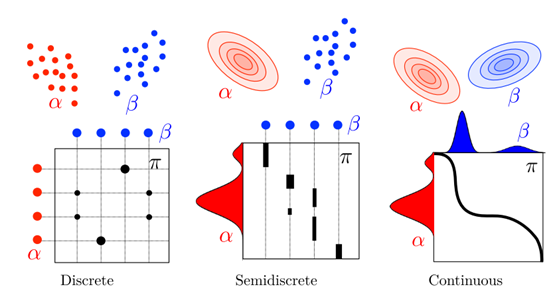
\includegraphics[width=0.5\hsize]{pic/ot}
	\caption{Different forms of Optimal Transport}
	\end{center}	
	\end{figure}			
	
\end{frame}


\begin{frame}
	\begin{screen}{Unbalanced Optimal Transport (UOT)}
\begin{equation}
\label{eq:uot}
\operatorname{UOT}(\vec{a},\vec{b}) :=  \min_{ \mat{T} \in \R_{+}^{m \times n},\lambda>0}\lambda \langle \mat{C}, \mat{T} \rangle + D_h(\mat{T} \one_m, \vec{a}) + D_h(\mat{T}^{\tranT} \one_n, \vec{b})
\end{equation}

\end{screen}
	
	\begin{itemize}
	\item Optimal Transport can only deal with balanced samples, a relaxed version with divergence function $D_h$ is required for more general applications.
	\item the most famous UOT solver is the Sinkhorn, which uses Kullback-Leibler divergence to penalize and add an entropy part $\eta H(\mathbf{T})$ onto the problem, its complexity is $O(\frac{n^2}{\epsilon})$ $\cite{DBLP:journals/corr/abs-2002-03293}$
	\item It is natural to consider whether other powerful optimizers exist.
	\end{itemize}
\end{frame}


\section{Algorithms}
\begin{frame}
\frametitle{The Lasso problem and the UOT problem}
	
	\begin{itemize}
	\item UOT has a similar structure to the Lasso problem:
$$
\begin{aligned}
\min_{\vec{t} \in \R_{+}^{mn}} f(t) := \min_{\vec{t} \in \R_{+}^{mn}}\lambda \vec{c}^{\tranT}\vec{t} + D_h(\mat{X}\vec{t},\vec{y})
\end{aligned}
$$
\item Lasso Problem:

\begin{equation}
\label{eq:uot}
\min_{\vec{t} \in \R^{mn}} f(t) := \min_{\vec{t} \in \R^{mn}} \lambda \|\vec{t}\| + D_h(\mat{X}\vec{t},\vec{y})
\end{equation}
\item $L_2$ or Kullback-Leibler divergence penalized UOT
$$
\begin{aligned}
f(t) &:= \lambda \vec{c}^{\tranT}\vec{t} + \|\mat{X}\vec{t}-\vec{y}\|_2^2\\
f(t) &:= \lambda \vec{c}^{\tranT}\vec{t} + KL(\mat{X}\vec{t},\vec{y})
\end{aligned}
$$
$y=[\vec{a}^{\tranT} \vec{b}^{\tranT}]^{\tranT}$ and $\mat{X}$, for example, when $n=3$, is:
\begin{align}
 \mat X= 
\begin{pmatrix}
1&1&1& & & & & &\\
 & & &1&1&1& & &\\
 & & & & & &1&1&1\\
1& & &1& & &1& &\\
 &1& & &1& & &1&\\
 & &1& & &1& & &1\\
\end{pmatrix}
\end{align}	
\end{itemize}
\end{frame}


\begin{frame}
\frametitle{The Lasso Problem and Dynamic Screening}
		\begin{screen}{Composite convex problem}
\begin{equation}
\min _{\vec{t} \in \mathbb{R}^{n}}\{d(\vec{t})+g(\vec{t})\}
\end{equation}
	\end{screen}	
\begin{itemize}
	\item For Lasso:
	$$
		d(\vec{t})= \|\mat{X}\vec{t}-\vec{y}\|_2^2, \quad g(\vec{t}) = \lambda \|\vec{t}\|
	$$
	
	\item For $L_2$ penalized UOT:
	$$
		d(\vec{t})= \|\mat{X}\vec{t}-\vec{y}\|_2^2, \quad g(\vec{t}) = \lambda \vec{c}^{\tranT}\vec{t}
	$$

	\item For Kullback-Leibler divergence penalized UOT:
	$$
		d(\vec{t})= KL(\mat{X}\vec{t},\vec{t}),\quad g(\vec{t}) =  \lambda \vec{c}^{\tranT}\vec{t}
	$$
\end{itemize}

\end{frame}


\begin{frame}
\frametitle{Screening}
	\begin{screen}{Motivation:}
	
	\quad Lasso-like regularizations cause a sparse solution $\operatorname{card}(\mat{T}_{ij}\|\mat{T}_{ij} = 0)\approx n^2$, for $\mat{T} \in \mathbb{R}^{m \times n}$. We identify the elements equal to zero theoretically and freeze them to save computational time.
	
	\end{screen}	
		\begin{itemize}
		\item As the UOT could be regarded as a Lasso-like problem, this technology can handle UOT as well.
	   	\end{itemize}
	\begin{figure}[htbp]
	\begin{center}	
	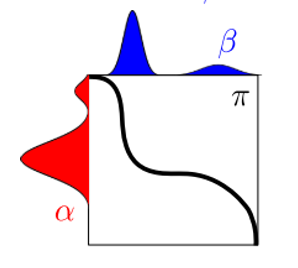
\includegraphics[width=0.3\hsize]{pic/sparse}
	\caption{The typical sparse solution for OT problem}
	\end{center}	
	\end{figure}	
	
\end{frame}


\begin{frame}
\frametitle{Dynamic Screening Framework}
	\begin{screen}{Frenchel-Rockafellar Duality \cite{NEURIPS2021_7b5b23f4}}
\begin{equation}
\begin{split}
	&P(t) = \min_{t} d(\mat{X}\vec{t}) + g(\vec{t})\\
	&D(\theta) = \max_{\theta} -d^{*}(-\theta) + g^{*}(\mat{X}^{\tranT}\theta)
\end{split}
\end{equation}
	\end{screen}	
		\begin{itemize}
		\item $d(\mat{X}\vec{t})$ is the distance measure like $L_2$ function and KL divergence.
		\item $g(\vec{t})$ is the Lasso-like sparse regularization such as $L_1$ penalty or optimal transport problem, we can convert it to constraints, then the dual problem is:  
	\end{itemize}
			$$
	\begin{aligned}
			&D(\theta) =  \max_{\theta}-d^{*}(-\theta)\\
			&\text{s.t.}\quad \forall i,\quad  h_{i}(\theta)\leq 0\\  
	\end{aligned}
		$$
\end{frame}

\begin{frame}
\frametitle{Screening}	
		\begin{itemize}
		 \item Relying on the KKT condition, we know that, for the optimum $\hat{\theta}$, we must have $\vec{\hat{t}}_i h_{i}(\hat{\theta})=0$. which indicates if $h_{i}(\hat{\theta})<0$, then $\vec{\hat{t}}_i=0$. 
		 \item For Lasso, the KKT condition is: 
		$$
		{h_{i}(\hat{\theta})=\|\vec{x}_i^{T}\hat{\theta}\| - 1 < 0}  \Rightarrow \vec{\hat{t}}_i = 0
		$$
		\item For UOT: 
		$$
		{h_{i}(\hat{\theta})=\vec{x}_i^{T}\hat{\theta} -\lambda \vec{c}_i \leq 0}  \Rightarrow \vec{\hat{t}}_i = 0
		$$
		\item However, we don't know the value of the optimum solution $\hat{\theta}$ at first.
		\item If we could find an area $R^{DS}$ containing the $\hat{\theta}$, we know that:
		$$
		h_{i}(\hat{\theta}) \leq \max_{\theta \in R^{DS}}h_{i}(\theta) 
		$$
		\item And if found that $ \max_{\theta \in R^{DS}}h_{i}(\theta) <0$, we can freeze the elements $\vec{\hat{t}}_i$ before we know the optimum solution.
		\end{itemize}
\end{frame}


\begin{frame}
\frametitle{Screening}	
		\begin{itemize}
		\item If we can find a $\tilde{\theta}$ that satisefied with the dual constrains, then we can construct an area $R^{DS}(\tilde{\theta})$, for $L_2$ penalized problem:
\begin{equation}
\begin{split}
	&\frac{1}{2}\| \theta -\tilde{\theta}\|_2^{2} + D(\tilde{\theta}) \leq D(\theta) \leq -d^{*}(-\theta) \\
	& \text{s.t. } g(\tilde{\vec{t}})-\theta^{T}\mat{X}\tilde{\vec{t}}< 0
\end{split}
\end{equation}
		\item The left part is strongly concave inequality and the right part is the dual inequality. 
		\item This area contains $\tilde{\theta}$ and the optimum $\hat{\theta}$
		\item If we could prove the $\max_{\theta \in R^{DS}(\tilde{\theta}) } h_{i}(\theta)<0$, then it holds for the optimum $\hat{\theta}$. It indicates that $ h_{i}(\hat{\theta})<0$, and the element $i$ of the primal optimal solution $\hat{\vec{t}}$ must be zero. 
		\end{itemize}
\end{frame}


\begin{frame}
\frametitle{Screening}
	\begin{figure}[htbp]
	\begin{center}	
	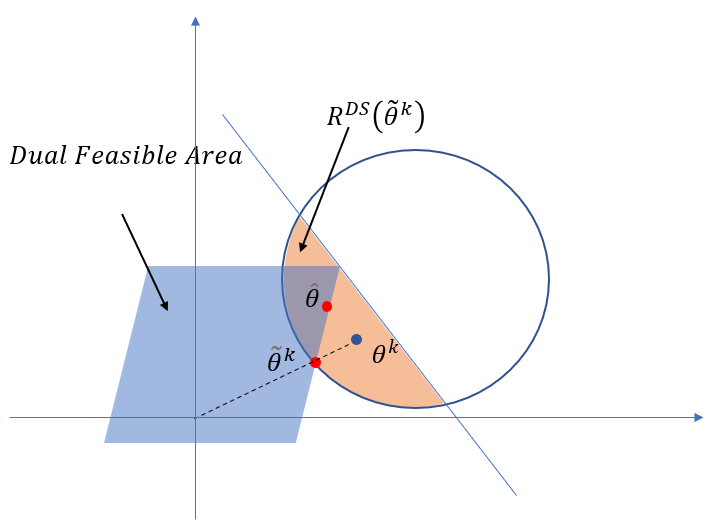
\includegraphics[width=0.8\hsize]{pic/proj}
	\caption{Projection in Screening}
	\end{center}	
	\end{figure}	
\end{frame}


\begin{frame}
\frametitle{Screening}
	\begin{itemize}
		\item We can dynamically compute an approximate solution $\theta^{k}$ by any algorithm and project it onto the dual constraints as $\tilde{\theta}^{k}$.
		\item We hope the projected $\tilde{\theta}^{k}$ could be closed enough to $\hat{\theta}$ to produce a smaller $R^{DS}(\tilde{\theta}^{k})$
		\item A smaller area can help us screen more variables as 
		$$
		\max_{\theta \in \tilde{R} \in R^{DS}(\tilde{\theta})}{\|\vec{x}_i^{T}\theta\|} \leq \max_{\theta \in R^{DS}(\tilde{\theta})}{\|\vec{x}_i^{T}\theta\|} 
		$$
		always holds.

	\end{itemize}
	
\end{frame}


\begin{frame}
\frametitle{The Projection method}
	\begin{itemize}
		\item The Lasso method is to shrink all $\tilde{\theta}$ together.
		$$
			\tilde{\theta} = \frac{\theta}{\max(1,\|\frac{\mat{X}^{T}\theta}{\vec{c}}\|_{\infty})}
		$$
	
		\item It is not suitable for the UOT problem as the cost value $c_{i}$ might be small and even zero. 
		\item We propose to use a shifting method, as the $x_{i}$ has a specific sparse structure which could rewrite the problem as:
		$$
		\theta_{i_{1}}+\theta_{i_{1}}<\vec{c}_i
		$$
		we decide to shift $\theta_{j}$ according to the maximum positive difference of $	\frac{\theta_{i_{1}}+\theta_{i_{1}}-\vec{c}_i}{2}$
	\end{itemize}
\end{frame}


\begin{frame}
\frametitle{The Projection method}
Shifting Screening method:
		$$
		\tilde{\theta}_{i}=\left\{
	\begin{aligned}
			&\theta_{i} -  \max_{j \mod{m} = i}&(\frac{\theta_{j_{1}}+\theta_{j_{2}}-\vec{c}_j}{2}) & 0\leq i<m\\
			&\theta_{i} -\max_{j \mid m = i}&(\frac{\theta_{j_{1}}+\theta_{j_{2}}-\vec{c}_j}{2})  & m\leq i<m+n
	\end{aligned}
	\right.
		$$
	\begin{figure}[htbp]
	\begin{center}	
	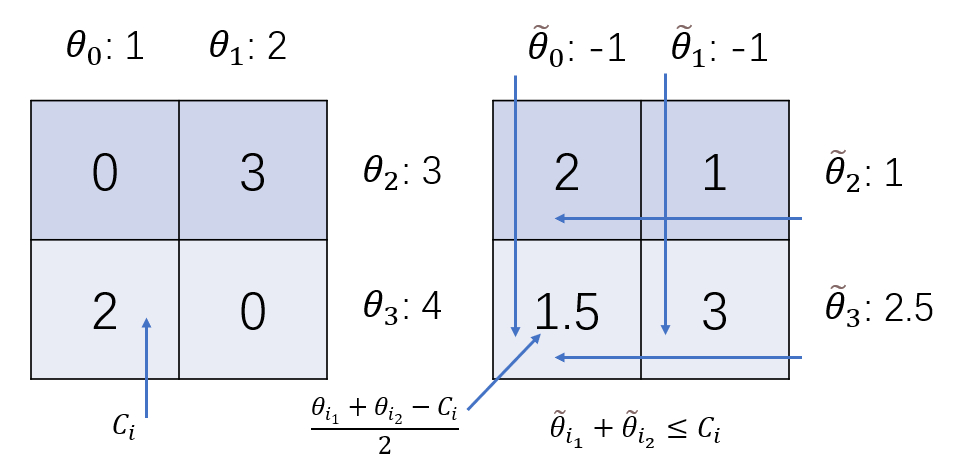
\includegraphics[width=0.8\hsize]{pic/shifting}
	\caption{Shifting on a 2$\times$2 matrix}
	\end{center}	
	\end{figure}

\end{frame}

\begin{frame}
\frametitle{The Projection Method}
	\begin{figure}[htbp]
	\begin{center}	
	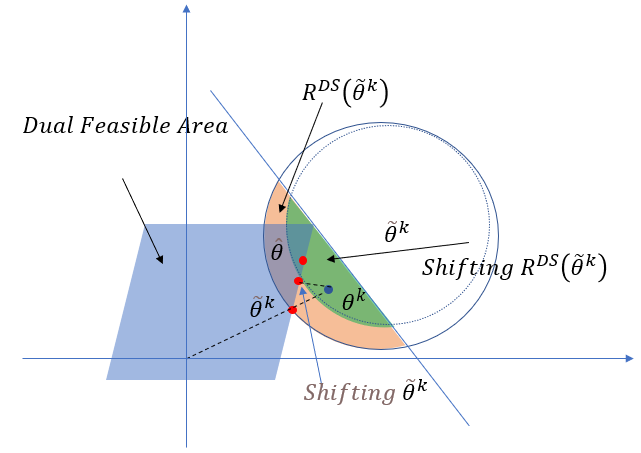
\includegraphics[width=0.8\hsize]{pic/new_proj}
	\caption{Difference of the projection method in Screening}
	\end{center}	
	\end{figure}

\end{frame}

\section{Experiments}
\begin{frame}
\frametitle{Experiments}
	\begin{figure}[htbp]
	\begin{center}	
	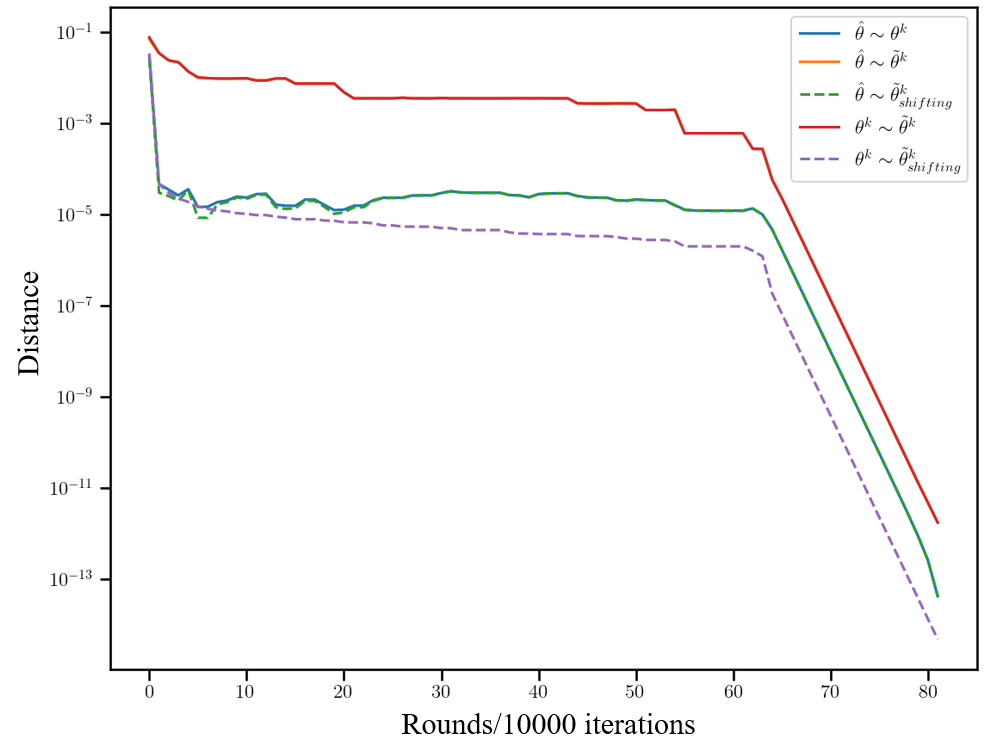
\includegraphics[width=0.8\hsize]{pic/dis}
	\caption{Distance between the projected point with $\hat{\theta}$ or $\theta^k$ }
	\end{center}	
	\end{figure}

\end{frame}


\begin{frame}
\frametitle{Experiments}
	\begin{figure}[htbp]
	\begin{center}	
	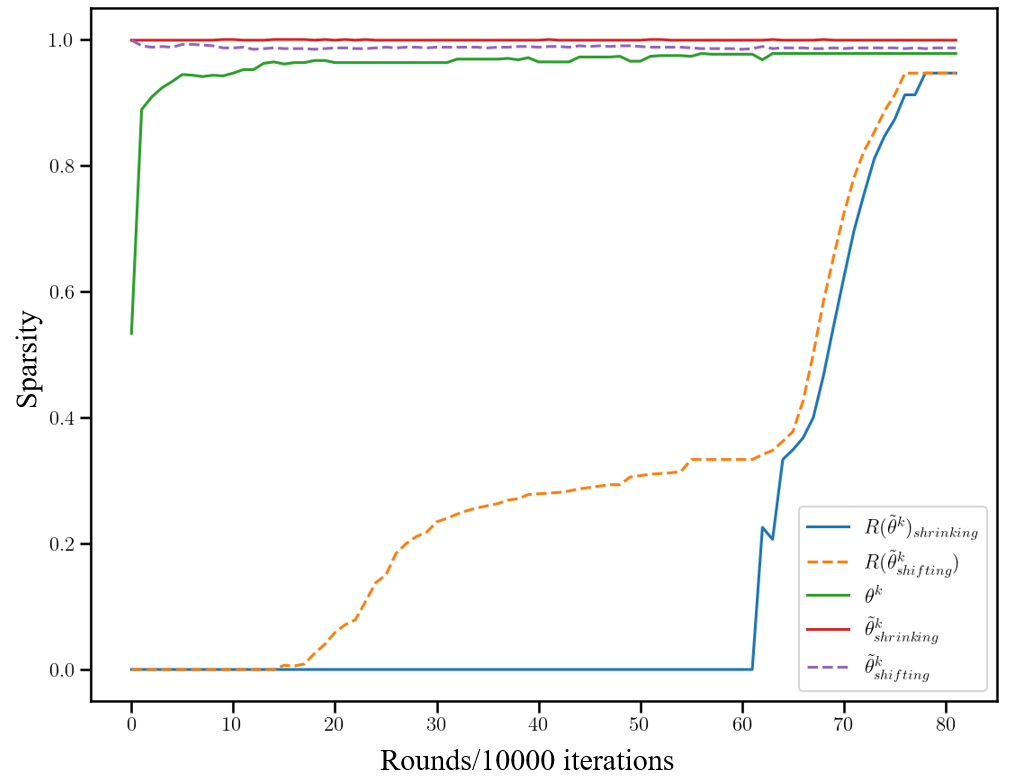
\includegraphics[width=0.8\hsize]{pic/spa}
	\caption{The Screening Ratio}
	\end{center}	
	\end{figure}

\end{frame}


\section{Prospect and Plan}
\begin{frame}
\frametitle{Potential and defects}
	\begin{itemize}	
	\item The UOT problem has the potential to screen out better due to its specific sparse structure of matrix $\mat{X}$.
	\item Screening is irrelevant to the optimization method you use and especially effective for the MM algorithm (which could be regarded as one kind of Mirror Descent)
	\item KL penalized Lasso problem also has a screening method \cite{9414183}, which could be applied to the KL penalized UOT problem, we might accelerate Sinkhorn Algorithm, which is only suitable for KL penalized UOT, with the Screening method. 
	\end{itemize}	
\end{frame}

\begin{frame}
\frametitle{Future Plan}
	\begin{itemize}
	\item We designed a new Two Planes Screening method to construct a new and smaller area $R^{T-DS}(\tilde{\theta})$, which further improve the screening ratio without adding much computational burden. We are writing papers and orgnizing experiments for AISTATS.
	\item We hope to generalizing the screening method to the KL penalized UOT problem and the Sinkhorn Algorithm.  
	\end{itemize}	
\end{frame}

\section{Reference}

\begin{frame}[allowframebreaks]
%\setbeamertemplate{bibliography item}[text]
\setbeamertemplate{bibliography item}[triangle]
        \frametitle{References}
        %\bibliographystyle{amsalpha}
        \bibliographystyle{apalike}
        \bibliography{sample}
\end{frame}


\begin{frame}
	\begin{center}	
	\vspace*{1.0cm}
	\IMPB{\Large ご清聴ありがとうございました. }	
	
	\vsp\vsp
	\IMPB{\Large Thank you for listening. }
	\vspace*{1.0cm}
	\end{center}	
	\vspace*{-0.5cm}
\end{frame}

\end{document}





